Bereits in den vorherigen Kapiteln wurde auf die Durchführung dieses Versuchs eingegangen. Im folgenden wird über den Ablauf und einige Problematiken gesprochen, welche sich während dem Herstellungs- und Laufprozess herauskristallisierten. 

Wie bereits in Kapitel \ref{Herstellung_MAP} beschrieben, wird zunächst das MAP hergestellt und anschließend in die Formen gegossen. Während der Vermengung wurde festgestellt, dass bei 60\,\%gem MAP die Durchmischung nicht gewährleistet werden kann, solang der verwendete Becher über die Hälfte voll ist. Deshalb wurden in diesem Fall zwei identische Proben hergestellt, welche erst in der Form zusammengegossen wurden. Alle anderen Proben mussten nach der Durchmischung in zwei separate Becher umverteilt werden, da während der Entgasung das Gemisch an Volumen bis zu einer Druckabnahme von etwa $15 \unit{mbar}$ zunimmt. Dies hat zur Folge, dass der Becher nur etwa halb voll sein darf, damit das MAP nicht \glqq überkocht\grqq{}. 

Nach spätestens 24 Stunden ist das Silikon vollständig ausgehärtet und kann aus der Form gelöst werden. Aufgrund der Einhängevorrichtung musste die Gussform hierbei aufgebrochen werden, um die nur $2 \unit{mm}$ dicken Stangen nicht abzubrechen oder aus dem MAP zu reißen. Zudem verkeilt sich das Silikon in den Unebenheiten des 3D Drucks, sodass selbst mithilfe von Silikonöl, welches vor dem Gießen in die Form gegeben werden kann, sich das MAP nur schwer lösen lässt. 



% Probleme bei der Herstellung
% Tatsächlicher Messablauf
% Keine Messung der Schräglage

\begin{figure}[tb]
	\hfill
	\begin{subfigure}[c]{0.35\linewidth}
		\centering
		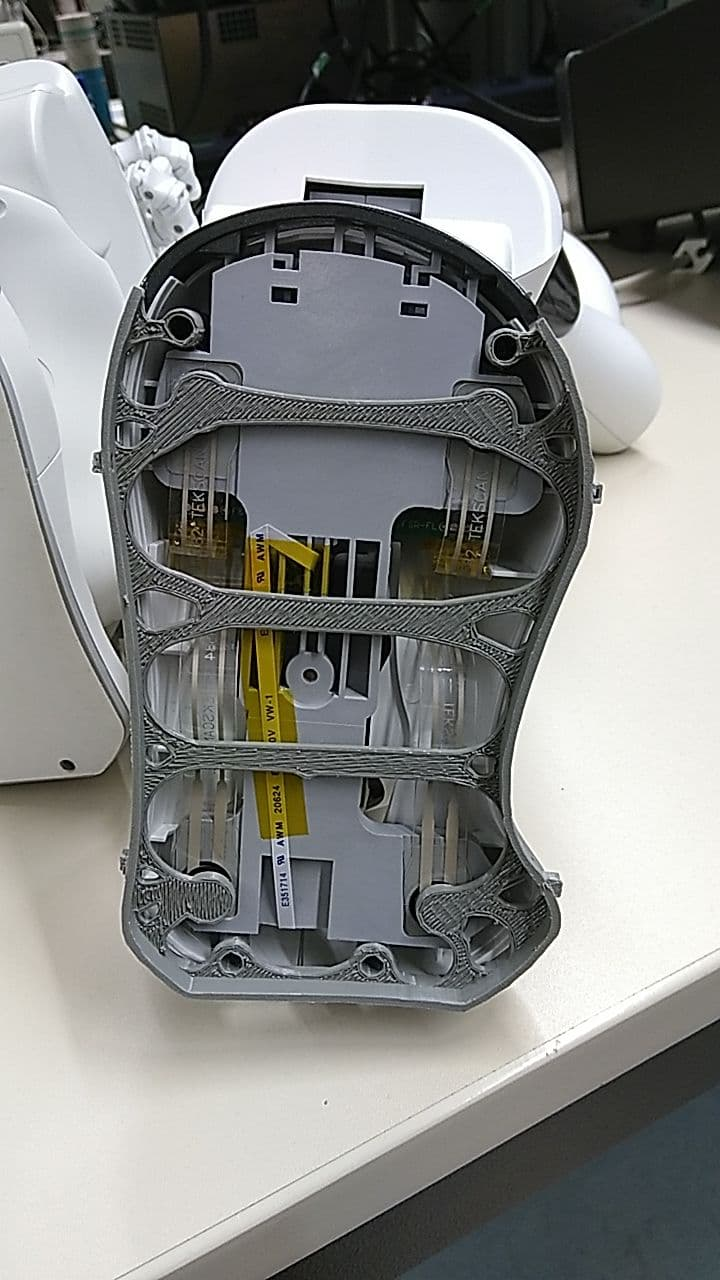
\includegraphics[width=\linewidth]{Bilder/Schuh_an_NAO_ohne_Sohle.jpg}
	\end{subfigure}
	\hfill
	\begin{subfigure}[c]{0.622\linewidth}
		\centering
		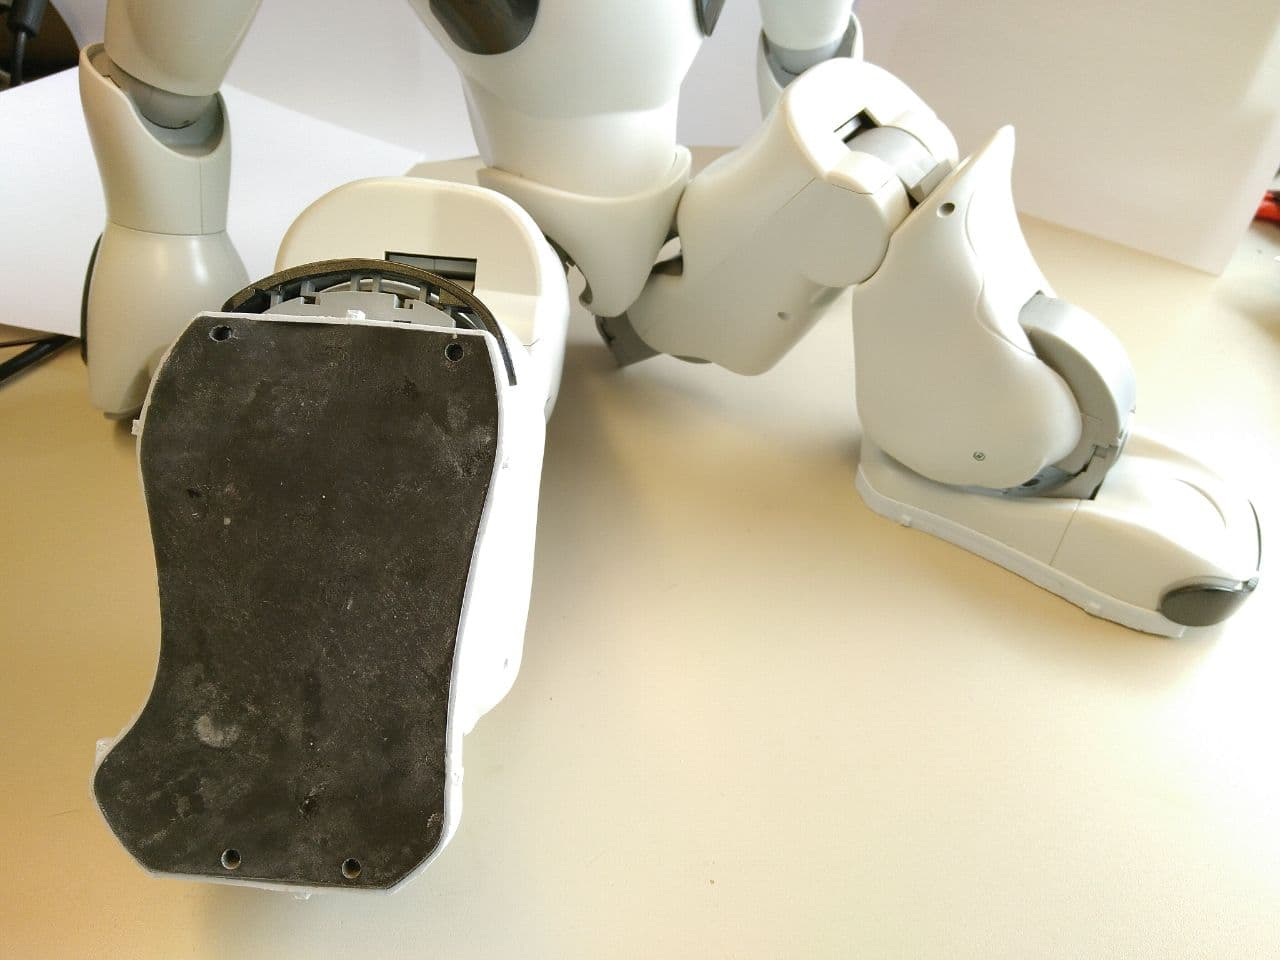
\includegraphics[width=\linewidth]{Bilder/Schuh_an_NAO_mit_Sohle.jpg}
	\end{subfigure}
	\hfill
	\caption{\textit{Links:} Der in Abb. \ref{Schuh_Inventor} in Autodesk Inventor erstellte Schuh aus PETG befestigt an der Unterseite des Fußes von NAO. \textit{Rechts:} Die aus der Gussform aus Abb. \ref{Gussform_Inventor} entnommene Sohle mit 20\,\% MAP Anteil befestigt in dem aus PETG gedruckten Schuh.}
	\label{nao_mit_schuhen}
\end{figure}

\begin{figure}[tb]
	\hfill
	\begin{subfigure}[c]{0.4\linewidth}
		\centering
		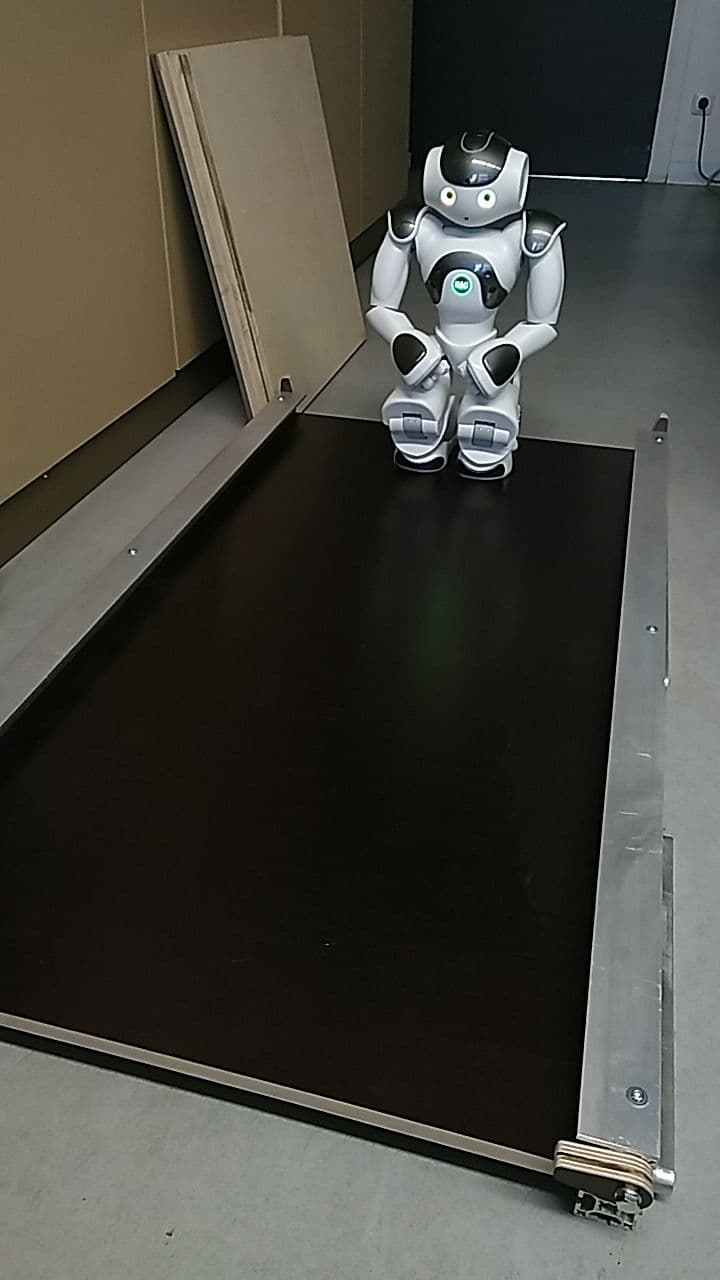
\includegraphics[width=\linewidth]{Bilder/NAO_auf_Rampe2.jpg}
	\end{subfigure}
	\hfill
	\begin{subfigure}[c]{0.4315\linewidth}
		\centering
		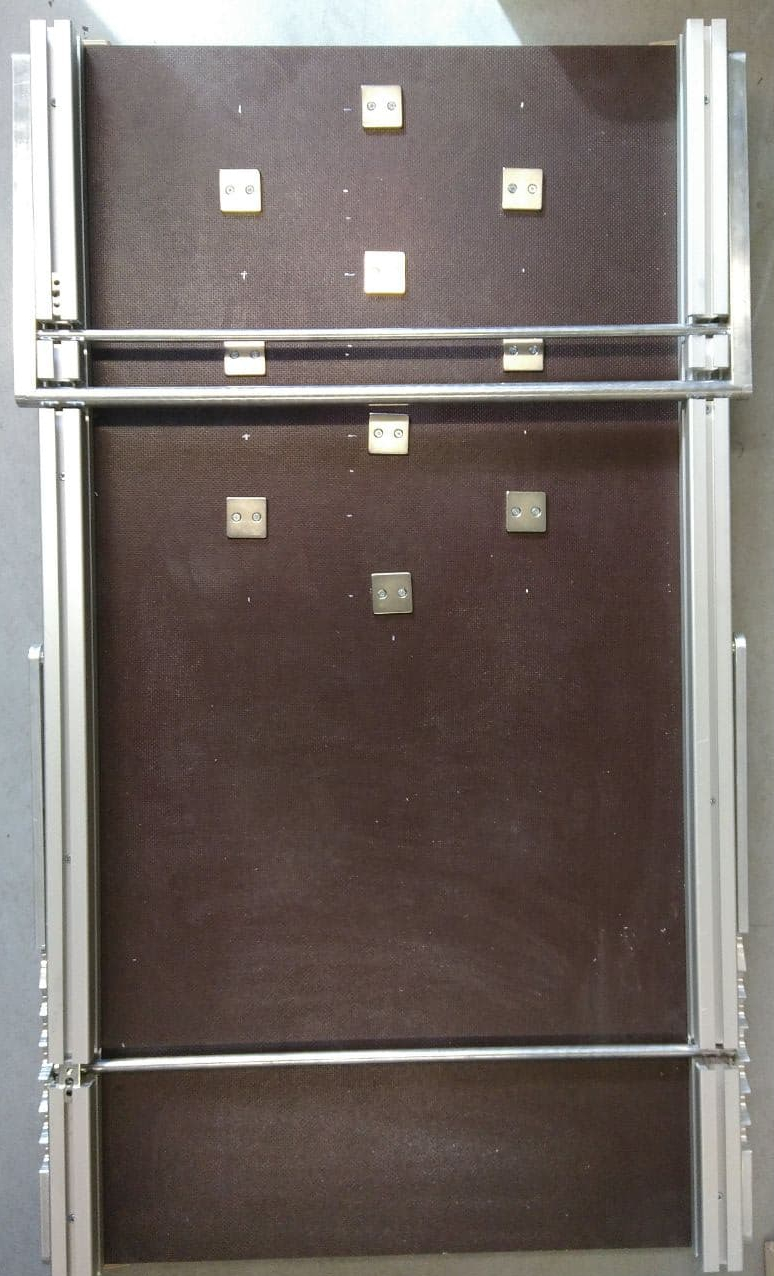
\includegraphics[width=\linewidth]{Bilder/magneten_an_rampe1_geschnitten.jpg}
	\end{subfigure}
	\hfill
	\caption{\textit{Links:} Der NAO Roboter steht im Ruhezustand an der Startposition auf der Rampe ohne Einlageplatten (an der Wand links neben NAO). \textit{Rechts:} Rampenunterseite mit befestigten Neodymmagneten.}
	\label{nao_und_rampe}
\end{figure}

